\documentclass{article}
\usepackage{graphicx} % Required for inserting images
% \usepackage[margin=2.54cm]{geometry}
\usepackage{amsmath} % For mathematical symbols and environments
\usepackage{hyperref}
\usepackage[backend=biber, style=numeric, citestyle=numeric, maxcitenames=1]{biblatex} %Imports biblatex package
\usepackage{mathtools}
\usepackage{physics}
\usepackage{placeins}
\usepackage[final]{listings}

\usepackage{xcolor}

\definecolor{backcolour}{RGB}{245,245,245}
\definecolor{commentcolour}{rgb}{0,0.6,0}
\definecolor{stringcolour}{rgb}{0.58,0,0.82}
\definecolor{white}{rgb}{1,1,1}



\lstloadlanguages{Python}
\lstdefinestyle{input}{
    keywordstyle=\color{blue},
    backgroundcolor=\color{backcolour},
    stringstyle = \color{stringcolour},
    commentstyle=\color{commentcolour},
    basicstyle=\ttfamily\small,
    breakatwhitespace=false,         
    breaklines=true,                 
    captionpos=b,                    
    keepspaces=true,                 
    numbers=none,                    
    numbersep=5pt,                  
    showspaces=false,                
    showstringspaces=false,
    showtabs=false,                  
    tabsize=2
  }
  
  \lstdefinestyle{output}{
    backgroundcolor=\color{white},
    keywordstyle = \color{black},
    basicstyle=\ttfamily\small,
    breakatwhitespace=false,         
    breaklines=true,                 
    captionpos=b,                    
    keepspaces=true,                 
    numbers=none,                    
    numbersep=5pt,                  
    showspaces=false,                
    showstringspaces=false,
    showtabs=false,                  
    tabsize=2
}
\lstset{
    style = input,
    language = Python
}

\addbibresource{dl-ref.bib} %Import the bibliography file

\title{Deep Learning}
\author{Mairi Hallman}
\date{May 2024}



\begin{document}

\maketitle

\newpage

\tableofcontents
\newpage

\section{Introduction}

\section{A Brief Overview of Tensors}

You are likely familiar with scalars, vectors, and matrices. These can be thought of as analagous data structures in zero, one, and two-dimensions, respectively. When generalizing to \(N\) dimensions, we refer to these collectively as tensors. A scalar is a zero-order tensor, a vector is a first-order tensor, and a matrix is a second-order tensor. A third-order tensor can be visualized as a stack of matrices. A fourth-order tensor would then be a vector of third order tensors. A fifth-order tensor is a matrix of third-order tensors... and so on.

% notation

% fiber and slices

\subsection{Tensor Products}

Tensor additon and subtraction are self-explanatory if matrix addition and subtraction are understood. The same cannot be said for tensor products. Below is an overview of tensor products necessary for the decompositions that will be presented in the next section.

\subsubsection{Outer Product \(\circ\)}

A tensor \(T^{(N)}\) can be expressed as a product of \(N\) vectors. This is called the outer product (denoted \(\circ\)).

\begin{equation}
    T^{(N)} = u_1 \circ u_2 \circ \dots \circ u_N
\end{equation}

% make less hand-wavey

\subsubsection{Kronecker Product \(\otimes\)}

The Konecker product of two matrices \(A\) and B, their Kronecker product is a matrix of the products of each element in \(A\) and the entire matrix \(B\).

\begin{equation}
    A \otimes B = \begin{bmatrix}
    a_{11}B & a_{12}B & \dots & a_{1n}B \\
    a_{21}B & a_{22}B & \dots & a_{2n}B \\
    \vdots & \vdots & \ddots & \vdots \\
    a_{m1}B & a{m2}B & \dots & a_{mn}B \end{bmatrix}
    \label{Kronecker} 
\end{equation}

\subsubsection{Khatri-Rao Product \(\odot\)}

The Khatri-Rao product of two matrices \(A\) and \(B\), each with the same number of columns, is a matrix composed of the Kronecker products of the columns in matrix \(A\) and the columns in matrix \(B\) with the same indices.

\begin{equation}
    A^{:\times n} \odot B^{:\times n} = \begin{bmatrix}
    a_{:,1} \otimes b_{:,1} & a_{:,2} \otimes b_{:,2} & \dots & a_{:,n} \otimes b_{:,n} \end{bmatrix}
    \label{Khatri-Rao}
\end{equation}

\subsubsection{Hadamard Product \(*\)}

The Hadamard product of two matrices \(A\) and \(B\) of the same dimensions is a matrix formed of the products of the elements in \(A\) and \(B\) with the same indices.

\begin{equation}
    A^{m \times n} * B^{m \times n} = \begin{bmatrix}
    a_{11}b_{11} & a_{12}b_{12} & \dots & a_{1n}b_{1n} \\
    a_{21}b_{21} & a_{22}b_{22} & \dots & a_{2n}b_{2n} \\
    \vdots & \vdots & \ddots & \vdots \\
    a_{m1}b_{m1} & a_{m2}b_{m2} & \dots & a_{mn}b_{mn} \end{bmatrix} 
    \label{Hadamard}
\end{equation}

\subsection{Tensor Decompositions}

% add intro

\subsubsection{CP Decomposition}

The canonical polyadic, or CP Decomposition, decomposes a tensor into vectors.

\begin{equation}
    T = \sum_{r-1}^R u_r^{(1)} \circ  u_r^{(2)} \circ \dots  u_r^{(R)}\
    \label{CP}
\end{equation} % review notation

% add info re computation

\subsubsection{Tucker Decomposition}

The Tucker decomposition decomposes a tensor into a core tensor and factored matrices. % add more explanantion

\begin{equation}
    T = C\prod_{n=1}^N A^n
    \label{Tucker}
\end{equation} % review notation

where \(C\) is the core tensor.

% add info re computation

\subsubsection{Tensor Train}

The tensor train decomposition decomposes a tensor into a product of third-order tensors. It is used when a tensor is too large for the CP decomposition to be practical. 

% add representative equation, info on computation


\section{Why Deep Networks} % see Probabilistic ML 13.2.5

Deep networks can often approximate complex functions with far fewer nodes than a shallow network. This is because the number of linear regions in the network grows exponentially with the number of layers \cite{montufar2014}.

To illustrate, consider a network with 5 layers, each with 10 nodes for a total of 50 nodes. For the sake of this example, we will assume that each layer has one input. The number of linear regions that can be learned by this network is \(10^5\). For a single-layer network to learn \(10^5\) linear regions, it would require \(10^5\) nodes. 

\subsection{Getting Started}

To help you get comfortable with neural network architecture, we will use Pytorch and Lightning code a network to complete a task that you are already very familiar with: linear regression. First, import dependencies and set a seed for reproductibility.

\lstinputlisting[firstline=18,lastline=24]{dl-scripts/introductory-ex.py}

Generate some dummy data according to the relationship \(y = 3x + 1\).

\lstinputlisting[firstline=28,lastline=31]{dl-scripts/introductory-ex.py}

Once the data loader has been initialized, define a class for our model.

\lstinputlisting[firstline=36,lastline=55]{dl-scripts/introductory-ex.py}

Now the fun part - training!

\lstinputlisting[firstline=59,lastline=61]{dl-scripts/introductory-ex.py}

\begin{lstlisting}[style=output]
INFO: GPU available: False, used: False
INFO:lightning.pytorch.utilities.rank_zero:GPU available: False, used: False
INFO: TPU available: False, using: 0 TPU cores
INFO:lightning.pytorch.utilities.rank_zero:TPU available: False, using: 0 TPU cores
INFO: HPU available: False, using: 0 HPUs
INFO:lightning.pytorch.utilities.rank_zero:HPU available: False, using: 0 HPUs
INFO: 
  | Name   | Type   | Params | Mode 
------------------------------------------
0 | linear | Linear | 2      | train
------------------------------------------
2         Trainable params
0         Non-trainable params
2         Total params
0.000     Total estimated model params size (MB)
1         Modules in train mode
0         Modules in eval mode
INFO:lightning.pytorch.callbacks.model_summary:
  | Name   | Type   | Params | Mode 
------------------------------------------
0 | linear | Linear | 2      | train
------------------------------------------
2         Trainable params
0         Non-trainable params
2         Total params
0.000     Total estimated model params size (MB)
1         Modules in train mode
0         Modules in eval mode
/usr/local/lib/python3.10/dist-packages/lightning/pytorch/loops/fit_loop.py:298: The number of training batches (10) is smaller than the logging interval Trainer(log_every_n_steps=50). Set a lower value for log_every_n_steps if you want to see logs for the training epoch.
Epoch 99: 100% [==============================] 10/10 [00:00<00:00, 50.34it/s, v_num=1]
INFO: `Trainer.fit` stopped: `max_epochs=100` reached.
INFO:lightning.pytorch.utilities.rank_zero:`Trainer.fit` stopped: `max_epochs=100` reached.
\end{lstlisting}

Let's see how our model did.

\lstinputlisting[firstline=65,lastline=66]{dl-scripts/introductory-ex.py}

\begin{lstlisting}[style=output]
Trained Model Parameters: Slope: 2.9757, Intercept: 0.9874
\end{lstlisting}

That's pretty good! In the coming sections, we will explore more advanced techniques for training deeper networks, as well as different specialized network arcitectures.

\section{Activation Functions and Weight Initialization for Hidden Layers} % see Deep Learning 6.3; Probabilistic ML 13.2.3

Different types of hidden units serve different purposes within deep networks. Most types of hidden units perform an affine  transformation on the layer's input, and then apply an activation function \(g(z)\) to the transformed inputs \cite{Goodfellow-et-al-2016}. If all activation functions within a deep network are linear, then the network reduces to a linear model \cite{pml1book}. While linear activation functions can be useful for reducing the number of parameters in a model , the discussion surrounding hidden units and their activation functions within a deep network typically concerns non-linear units \cite{Goodfellow-et-al-2016}. 

\subsection{ReLU}

In modern deep networks, the default most commonly used activation function for hidden layers is the rectified linear unit, or ReLU activation function.

\begin{equation}
    a(z) = max(0, z)
    \label{ReLU-activation}
\end{equation}

This is analagous to a linear activation function with negative inputs "turned off" \cite{pml1book}. 

Notice that this function isn't differentiable at zero. In theory, this should make ReLU useless for gradient-based learning. In practice, most deep networks don't achieve a loss of zero, so this typically isn't a problem.

Variations of ReLU typically modify the slope for negative inputs \cite{Goodfellow-et-al-2016}. For a given input \(z_i\), this can be generalized as

\begin{equation}
    a(z,\alpha)_i = max(0, z_i) + \alpha_i min(0,z_i)
    \label{generalization-ReLU}
\end{equation}

Several ReLU variations of this form are listed below.

\paragraph{Absolute Value Rectification}\(\alpha = -1\); commonly used for image processing \cite{Goodfellow-et-al-2016}.

\paragraph{Leaky ReLU}\(\alpha\) is a small positive value. Leaky ReLU is used in place of standard ReLU to prevent the "dying ReLUs" problem. Units using ReLU as an activation "die" when all of the inputs are non-positive. All negative inputs results in all zero outputs, and the weights can't be updated \cite{hands-on-ml}.

\paragraph{Parametric Leaky ReLU}Leaky ReLU where \(alpha\) is learned by the model \cite{hands-on-ml}.

\subsection{The Sigmoid and Hyperbolic Tangent Functions}

In the early days of deep learning, two commonly used activation functions for hidden units were the sigmoid function

\begin{equation}
    a(z) = \sigma (z) = \frac{1}{1 + e^{-z}}
    \label{sigmoid-activation}
\end{equation}

and the hyperbolic tangent function

\begin{equation}
    a(z) = tanh(z)
    \label{tanh-activation}
\end{equation}

These activation functions are no longer recommended for hidden units because they saturate. The sigmoid function saturates at zero and one, and the hyperbolic tangent function saturates at  negative one and one. Saturation is problematic because it leads to the gradient of a layer's output with respect to its input. Recall what we know about backpropagation from section 21.4.3. If the gradient is close to zero, the weights will update very slowly, if at all. Without a gradient, the model can't converge to a solution. This phenomenon is known as the vanishing gradient problem.

\subsection{Weight Initialization} % PML1 13.4.5.1

As mentioned in chapter 21, before a deep network can be trained, its weights have to be randomly initialized. Proper initialization of weights is crucial for fast convergence and preventing exploding gradients. Random weights are often sampled from a normal distribution. If the variance of this distribution is fixed for all layers, gradients may explode during training \cite{pml1book}. It is therefore reccommended to use one of the weight initialization strategies below.

\paragraph*{Glorot Initialization}, also know as Xavier initialization, sets the variance of the sampling distribution for each layer to \(\sigma^2 = \frac{2}{n_{in} + n_{out}}\), where \(n_in\) is the number of input connections to a unit in the layer, and \(n_out\) is the number of output connections. This is the preferred initialization scheme for sigmoid activation \cite{pml1book} and, by extension, hyperbolic tangent activation.

\paragraph*{LeCunn Initialization} uses a variance of \(\sigma^2 = \frac{1}{n_{in}}\), and is identical to Glorot initialization with an equal number of input and output connections \cite{pml1book}.

\paragraph*{He Initialization} uses a variance of \(\sigma^2 = \frac{2}{n_{in}}\), and is the preferred initialization scheme for ReLU activation. 

\section{Regularization} % see DL all 7.1, 7.6, maybe 7.7, 7.8, probably 7.9, 7.12; Probabilistic ML 13.5

\subsection{Weight Decay} % L2: DL 7.1.1, PML1 13.5.2 and L1: DL 7.1.2

Recall ridge and LASSO regression from section 20.2.4. When generalized beyond linear models, these regularization techniques are known respectively as \(\it{L}^2\) and \(\it{L}^1\) regularization. In the context of neural networks, these methods are both commonly referred to as weight decay. Weight decay applies a regularization term to the objective function \(J(\vb*{w})\). The regularized objective function \(\tilde{J}(\vb*{w})\) is 

\begin{equation}
    \tilde{J}(\vb*{w}) = J(\vb*{w}) +\frac{\lambda}{2}\norm{w}^2_2
    \label{L2-reg}
\end{equation} for \(\it{L}^2\) weight decay, and 

\begin{equation}
    \tilde{J}(\vb*{w}) = J(\vb*{w}) +\lambda\norm{w}_1
    \label{L1-reg}
\end{equation} for \(\it{L}^1\) weight decay, where \(\lambda\) is a hyperparameter.

\subsection{Early Stopping} % DL 7.8

If a model is trained for too many epochs, the validation set error will reach a minumum at the optimal number of epochs, and then begin to increase as a result of overfitting. This can be prevented by implementing early stopping. When early stopping is used, a copy of the model's parameters is only saved at the end of a training iteration if the validation loss improves \cite{Goodfellow-et-al-2016}. Training stops automatically if the validation loss hasn't decreased, or has only decreased by a very small amount, after a given number of training loops.

\subsection{Dropout} % DL 7.12, PML 13.5.4

Dropout is a regularization technique that randomly sets a given proportion of the models weights to zero after each gradient step. This means that for each epoch, a "different" model is being trained \cite{Srivastava14}. This is similar to bagging, but instead of being independent, each model's weights are a subset of the full network's weights \cite{Goodfellow-et-al-2016}.

Dropout helps prevent overfitting by stopping units from becoming ``lazy". Consider a hockey team consisting of a few star players, many average players, and some weak players. Typically, the best players get the most playing time. The downside of this is that the others get less practice, and therefore don't improve at the same rate. If, for each game, a certain number of players were randomly selected and told to stay hom, the rest of the team would have to adapt to play without those players. In this scenario, the team is less at risk of becoming dependent on a few superstars, and the benchwarmers get a chance to improve and contribute. In this example, the team is the model, and each player is a unit. By randomly "dropping out" some players, the others get more practice and become better assets to the team \cite{hands-on-ml}.

\begin{figure}[h]
    \centering
    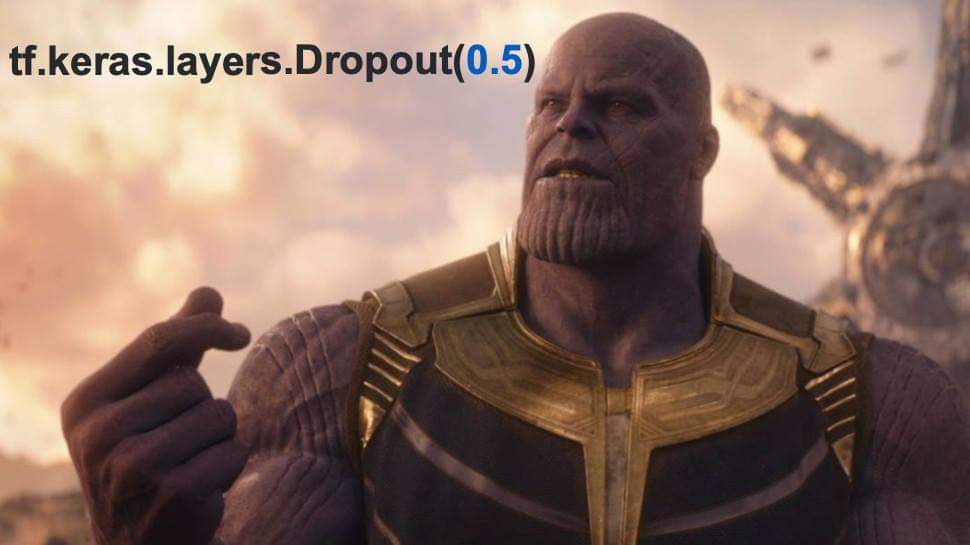
\includegraphics[scale = 0.24]{dl-figures/thanos-dropout-meme.jpg}
    \caption{Consider this meme from user @mlinterview on X. In the Marvel series, Thanos is a villain whose goal is to make half of all living organisms in the universe disappear. Those who disappear are randomly selected. While Thanon's motivations are not related to regularization, do you think this would force the remaining life forms to adapt for the better? Why or why not?}
    \label{figure:thanos-dropout-meme}
\end{figure}

\FloatBarrier

Please note that Thanos was unpopular for a reason; dropping out 50\% of the weights is very excessive and not advised \cite{tensorflow2015-whitepaper}.

\FloatBarrier

\section{Variants of Stochastic Gradient Descent} % See Deep Learning all 8.3, 8.4, all 8.5, 8.7.1, 8.7.4

In section 21.4.3, we introduced stochastic gradient descent. Below are some common variants of SGD.

\subsection{Momentum} % DL 8.3.2

A significant drawback of SGD is that it can be very slow to converge to an optimal solution. SGD with momentum helps address this by adding a weighted moving average of the past gradients. This allows the algorithm to converge more quickly when sequential gradients move in the same direction, and to slow down if there is a sudden change \cite{pml1book}. 

The momentum algorithm is implemented as follows. Here, \(\vb*{m}_t\) is the momentum, \(\eta\) is the learning rate, \(\vb*{g}_{t-1}\) is the gradient at previous output, and \(\vb*{\theta}_t\) is the output. \(\beta\) is the momentum hyperparamenter, which controls the exponential decay of the weights of past gradients. Common values of \(\beta\) are \(0.5\), \(0.9\), and \(0.99\) \cite{pml1book}

% \eta or \eta_t ?


\begin{align*}
    \vb*{m}_t &= \beta \vb*{m}_{t-1} + \vb*{g}_{t-1} \\
    \vb*{\theta}_t &= \vb*{\theta}_{t-1} - \eta \vb*{m}_t
\end{align*}


Some resources give a different set of formulas for optimization with momentum. Note that the following are equivalent when \(\vb*{m}_1 = 0\).

\begin{align*}
    \vb*{m}_t &= \beta \vb*{m}_{t-1} - \eta \vb*{g}_t \\
    \vb*{\theta}_t &= \vb*{\theta}_{t-1} + \vb*{m}_t
\end{align*}

\subsection{Nesterov Momentum}

An improved variant of the momentum algorithm was introduced in 2013 \cite{sutskever13}. This version, known as Nesterov momentum, uses the gradient at \(\vb*{\theta}_{t-1} + \beta \vb*{m}_{t-1}\) instead of at \(\theta{t-1}\). This can be thought of as an ``extrapolation" step. Instead of measuring at the previous output, we are assuming that the algorithm will continue to converge slightly ahead of this output with respect to the momentum. This allows for faster convergence.

\begin{align*}
    \vb*{g}_{t} &= \nabla \mathcal{L} (\vb*{\theta}_{t} + \beta \vb*{m}_{t}) \\
    \vb*{m}_{t+1} &= \beta \vb*{m}_{t} - \eta \vb*{g}_t \\
    \vb*{\theta}_{t+1} &= \vb*{\theta}_t + \vb*{m}_{t+1}
\end{align*}

% adaptive learning rate algorithms start here

\subsection{AdaGrad} % DL 8.5.1

Until now, our discussion of learning algorithms has concerned algorithms with static learning rates. The AdaGrad algorithm modifies the learning rates of the model parameters by dividing them by the square root of the Kronecker product of the vector of past gradients with itself. This speeds up convergence when the gradient is less extreme. 

The algorithm is provided below. The variable \(s\) is the gradient accumulation variable, with \(r_1 = 0\). \(\eta\) is the global learning rate, and \(\epsilon\) is a very small value to prevent division by \(0\).

\begin{align*}
    \vb*{s}_t &= \vb*{s}_{t-1} + \sqrt{\vb*{g}_t \otimes \vb*{g}_t} \\
    \vb*{\Delta \theta}_t &= \frac{-\eta}{\epsilon + \vb*{s_t}} \otimes \vb*{g} \\
    \vb*{\theta}_t &= \vb*{\theta}_{t-1} + \vb*{\Delta \theta}_t
\end{align*}

\subsection{RMSProp} % DL 8.5.2

RMsProp is similar to AdaGrad, but with an exponentially decaying moving average gradient accumulation variable \cite{Goodfellow-et-al-2016}. This allows the algorithm to converge more quickly as it approaches a solution.

The parameters here are the same as for AdaGrad, with the addition of \(\beta\) for the decay rate. A common value for \(\beta\) is 0.9 \cite{pml1book}.

\begin{align*}
    \vb*{s}_t &= \beta \vb*{s}_{t-1} + (1-\beta)\vb*{g}_t \otimes \vb*{g}_t \\
    \vb*{\Delta \theta}_t &= \frac{-\eta}{\epsilon + \vb*{s_t}} \otimes \vb*{g}_t \\
    \vb*{\theta}_t &= \vb*{\theta}_{t-1} + \vb*{\Delta \theta}_t
\end{align*}

\subsection{Adadelta} % need to find source

Adadelta is a variant of RMSProp that multiplies the update by an exponetially weighted moving average of the past updates \(\vb*{\delta}_t = \beta \vb*{\delta}_{t-1} + (1-\beta)(\vb*{\delta}_t)^2\) \cite{pml1book} \cite{zeiler2012}.

\begin{align*}
    \vb*{s}_t &= \beta \vb*{s}_{t-1} + (1-\beta)\vb*{g}_t \otimes \vb*{g}_t \\
    \vb*{\Delta \theta}_t &= \frac{-\eta \sqrt{\vb*{\delta}_{t-1}}}{\epsilon + \vb*{s_t}} \otimes \vb*{g}_t \\
    \vb*{\theta}_t &= \vb*{\theta}_{t-1} + \vb*{\Delta \theta}_t
\end{align*}

\subsection{Adam} % DL 8.5.3

The adaptive moment estimation, or Adam optimizer, can be thought of as a hybrid of the momentum and RMSProp algorithms. It is good practice to correct \(m_t\) and \(s_t\) for bias to prevent bias towards smaller values \cite{pml1book}. % add more
\begin{align*}
    \vb*{m}_t &= \beta_1 \vb*{m}_{t-1} + (1-\beta_1)\vb*{g}_{t-1} \\
    \vb*{s}_t &= \beta_2 \vb*{s}_{t-1} + (1-\beta_3)\vb*{g}_t \otimes \vb*{g}_t \\
    \hat{\vb*{m}}_t &= \frac{\vb*{m}_t}{1-\beta^t_1} \\ 
    \hat{\vb*{s}}_t &= \frac{\vb*{s}_t}{1-\beta^t_2} \\ 
    \vb*{\Delta \theta}_t &= \frac{-\eta}{\epsilon + \vb*{s_t}} \otimes \vb*{m}_t \\
    \vb*{\theta}_t &= \vb*{\theta}_{t-1} + \vb*{\Delta \theta}_t
\end{align*}

\section{Convolutional Neural Networks}

% add intro

\subsection{What Is Convolution?}

Many young people who are active on social media use filters on their pictures before posting them. These filters apply different effects to the photo, such as blurring, making the image black and white, or adding cartoon-like effects. When you apply a filter to a photo, you are using convolution. Convolution is an operation that takes the aggregation of the element-wise product of a tensor of input data and a (typically smaller) tensor, called a kernel. This produces a feature map. In the context of image processing, the original image is the input data, the filter is the kernel, and the filtered image is the feature map. 

This is an example of discrete convolution, which is the case that we will be primarily concerned with. % In the interest of providing a complete resource, equations for discrete and continuous convolution in one dimension are provided below \cite{Goodfellow-et-al-2016}.

In one dimension, discrete convolution is denoted
\begin{equation}
    \underbrace{s(i)}_{\substack{\text{feature} \\ \text{map}}} = (x*y)(i) = \sum\limits_{\substack{m}} \underbrace{x(m)}_{\substack{\text{input} \\ \text{data}}}\underbrace{y(i-m)}_\text{kernel}
    \label{1D-discrete-convolution}\
\end{equation}


% In the continuous case, equation \ref{1D-discrete-convolution} becomes
% \begin{equation}
    % s(i) = (x*y)(i) = \int_m x(m)y(i-m)dm
    % \label{1D-continuous-convolution}\
% \end{equation}

One of the most common applications of CNNs is in digital image processing. In the case of a black and white image, the input data is a two-dimensional tensor. Discrete convolution in two dimensions can be performed as follows \cite{Goodfellow-et-al-2016}. %check this

\begin{equation}
    s(i,j) = (x*y)(i,j)\sum\limits_{\substack{m}}\sum\limits_{\substack{n}} x(i,j)y(i-m,j-n)
    \label{2D-discrete-convolution}
\end{equation}

Since convolution is commutative, the following also holds. 

\begin{equation}
    s(i,j) = (y*x)(i,j)\sum\limits_{\substack{m}}\sum\limits_{\substack{n}} x(i-m,j-n)y(i,j)
    \label{flipped-2D-discrete-convolution}
\end{equation}

Two-dimensional discrete convolution is equivalent to reversing the row and column indices of the kernel, performing element-wise multiplication, and taking the sum of the products. In the context of deep learning, the term ``convolution" often refers to a similar operation called cross-correlation (equation). This is equivalent to convolution without the reversing of the matrix indices \cite{Goodfellow-et-al-2016}. 

\begin{equation}
    s(i,j) = (y*x)(i,j)\sum\limits_{\substack{m}}\sum\limits_{\substack{n}} x(i+m,j+n)y(i,j)
    \label{cross-correlation}
\end{equation}

\subsection{How Convolution is Used in Deep Neural Networks}

Since one kernel can only extract one feature, each convolutional layer in a network uses multiple kernels. CNNs can be very computationally expensive to train, so we often skip over positions in the kernels to reduce training time. The width of the kernel and the size of the output can also be controlled by zero padding the input. Without zero padding, the output of each later would continue to shrink. The number of rows/columns per convolution is referred to as the stride of the convolution operation \cite{Goodfellow-et-al-2016}. % check this


\subsection{The Convolutional Layer}

The convolutional layers used in a CNN have three steps \cite{Goodfellow-et-al-2016}.

\begin{enumerate}
    \item Several parallel convolutions yield a set of linear activations.
    \item Each linear activation function is run through a non-linear activation function, such as ReLU. This introduces non-linearity and gives the network more flexibility. % fact-check this
    \item A pooling function replaces the output at a given location with a summary statistic of nearby outputs. One common pooling function is the max pooling function, which provides the maximum output within a rectangular neighbourhood. Pooling is useful when we only care about whether a feature is present and not its specific location. It is also helpful when processing different-sized inputs.
\end{enumerate}

The output of each layer is then used as input to the next layer.
% discrete case: \((a * b)_n = \sum\limits_{\substack{i,j \\ i+j=n}} a_i \cdot b_j\)

\subsection{Image Classification Example}

In this example, we will use convolutional neural networks to perform image classification on the Rock Paper Scissors dataset. Other coding examples in this chapter use Pytorch and Lightning, but this example will use Tensorflow and Keras. While Pytorch is becoming the dominant Python framework for machine learning, Tensorflow is still a popular choice for deployment in industry. Using Tensorflow for this example also allows us to leverage the Tensorflow datasets library to fetch our data.

\lstinputlisting[firstline=14, lastline=21 ]{dl-scripts/cnn-ex1-colab.py}

The dataset is only partitioned into training and test sets, so we set aside 30\% of the training set as a validation set.

\lstinputlisting[firstline=25, lastline=30]{dl-scripts/cnn-ex1-colab.py}

Next, we normalize by dividing by 255 and resize the images to 128x128. We also shuffle the training data to ensure that the model doesn't learn its order, and batch the training, validation, and test data.

\lstinputlisting[firstline=34, lastline=44]{dl-scripts/cnn-ex1-colab.py}

We start with a simple network with one comvolutional layer with 16 filters and a 3x3 kernel.

\lstinputlisting[firstline=48,lastline=62]{dl-scripts/cnn-ex1-colab.py}

Before fitting our model, we add an early stop mechanism to prevent overfitting.

\lstinputlisting[firstline=66,lastline=75]{dl-scripts/cnn-ex1-colab.py}

\begin{lstlisting}[style=output]
Epoch 1/10
56/56 [==============================] - 10s 85ms/step - loss: 1.0240 - accuracy: 0.7137 - val_loss: 0.2209 - val_accuracy: 0.9563
Epoch 2/10
56/56 [==============================] - 5s 61ms/step - loss: 0.0743 - accuracy: 0.9881 - val_loss: 0.0240 - val_accuracy: 0.9947
Epoch 3/10
56/56 [==============================] - 4s 37ms/step - loss: 0.0131 - accuracy: 0.9989 - val_loss: 0.0148 - val_accuracy: 0.9947
Epoch 4/10
56/56 [==============================] - 4s 37ms/step - loss: 0.0045 - accuracy: 1.0000 - val_loss: 0.0062 - val_accuracy: 0.9987
Epoch 5/10
56/56 [==============================] - 5s 58ms/step - loss: 0.0020 - accuracy: 1.0000 - val_loss: 0.0042 - val_accuracy: 1.0000
Epoch 6/10
56/56 [==============================] - 4s 38ms/step - loss: 0.0013 - accuracy: 1.0000 - val_loss: 0.0039 - val_accuracy: 1.0000
Epoch 7/10
56/56 [==============================] - 4s 38ms/step - loss: 0.0010 - accuracy: 1.0000 - val_loss: 0.0041 - val_accuracy: 0.9987
Epoch 8/10
53/56 [===========================>..] - ETA: 0s - loss: 8.3814e-04 - accuracy: 1.0000Restoring model weights from the end of the best epoch: 5.
56/56 [==============================] - 5s 59ms/step - loss: 8.2481e-04 - accuracy: 1.0000 - val_loss: 0.0032 - val_accuracy: 0.9987
Epoch 8: early stopping
\end{lstlisting}

Training accuracy of 100\% and validation accuracy of over 99\%? If something seems too good to be true, it probably is. Let's evaluate on the test data.

\lstinputlisting[firstline=79,lastline=79]{dl-scripts/cnn-ex1-colab.py}

\begin{lstlisting}[style=output]
12/12 [==============================] - 1s 104ms/step - loss: 1.3345 - accuracy: 0.7151
[1.3345420360565186, 0.7150537371635437] 
\end{lstlisting}

As expected, no such luck. What happens when we add another convolutional layer?

\lstinputlisting[firstline=83,lastline=98]{dl-scripts/cnn-ex1-colab.py}

\begin{lstlisting}[style=output]
 Epoch 1/10
 56/56 [==============================] - 6s 43ms/step - loss: 1.4043 - accuracy: 0.5890 - val_loss: 0.4816 - val_accuracy: 0.9206
 Epoch 2/10
 56/56 [==============================] - 5s 54ms/step - loss: 0.2150 - accuracy: 0.9552 - val_loss: 0.0609 - val_accuracy: 0.9881
 Epoch 3/10
 56/56 [==============================] - 4s 38ms/step - loss: 0.0441 - accuracy: 0.9909 - val_loss: 0.0182 - val_accuracy: 0.9987
 Epoch 4/10
 56/56 [==============================] - 4s 39ms/step - loss: 0.0143 - accuracy: 0.9977 - val_loss: 0.0076 - val_accuracy: 0.9987
 Epoch 5/10
 56/56 [==============================] - 5s 60ms/step - loss: 0.0053 - accuracy: 0.9994 - val_loss: 0.0030 - val_accuracy: 1.0000
 Epoch 6/10
 56/56 [==============================] - 4s 41ms/step - loss: 0.0022 - accuracy: 1.0000 - val_loss: 0.0019 - val_accuracy: 1.0000
 Epoch 7/10
 56/56 [==============================] - 4s 39ms/step - loss: 0.0016 - accuracy: 1.0000 - val_loss: 0.0013 - val_accuracy: 1.0000
 Epoch 8/10
 56/56 [==============================] - 5s 60ms/step - loss: 9.5238e-04 - accuracy: 1.0000 - val_loss: 0.0011 - val_accuracy: 1.0000
 Epoch 9/10
 56/56 [==============================] - 4s 38ms/step - loss: 6.9435e-04 - accuracy: 1.0000 - val_loss: 8.4804e-04 - val_accuracy: 1.0000
 Epoch 10/10
 56/56 [==============================] - 4s 38ms/step - loss: 5.3139e-04 - accuracy: 1.0000 - val_loss: 7.7833e-04 - val_accuracy: 1.0000
\end{lstlisting}

\lstinputlisting[firstline=100,lastline=100]{dl-scripts/cnn-ex1-colab.py}

\begin{lstlisting}[style=output]
12/12 [==============================] - 0s 16ms/step - loss: 1.0663 - accuracy: 0.7634
[1.0662583112716675, 0.7634408473968506]
\end{lstlisting}

An improvement, but still not amazing. Would a third convolutional layer help?

\lstinputlisting[firstline=104,lastline=121]{dl-scripts/cnn-ex1-colab.py}


\begin{lstlisting}[style=output]
 Epoch 1/10
 56/56 [==============================] - 7s 44ms/step - loss: 0.6999 - accuracy: 0.7035 - val_loss: 0.1999 - val_accuracy: 0.9101
 Epoch 2/10
 56/56 [==============================] - 4s 39ms/step - loss: 0.0600 - accuracy: 0.9864 - val_loss: 0.0188 - val_accuracy: 0.9934
 Epoch 3/10
 56/56 [==============================] - 5s 53ms/step - loss: 0.0240 - accuracy: 0.9949 - val_loss: 0.0071 - val_accuracy: 1.0000
 Epoch 4/10
 56/56 [==============================] - 4s 39ms/step - loss: 0.0022 - accuracy: 1.0000 - val_loss: 0.0011 - val_accuracy: 1.0000
 Epoch 5/10
 56/56 [==============================] - 4s 41ms/step - loss: 7.2477e-04 - accuracy: 1.0000 - val_loss: 7.4349e-04 - val_accuracy: 1.0000
 Epoch 6/10
 56/56 [==============================] - 5s 63ms/step - loss: 4.0359e-04 - accuracy: 1.0000 - val_loss: 3.2628e-04 - val_accuracy: 1.0000
 Epoch 7/10
 52/56 [==========================>...] - ETA: 0s - loss: 2.2042e-04 - accuracy: 1.0000Restoring model weights from the end of the best epoch: 4.
 56/56 [==============================] - 4s 39ms/step - loss: 2.1410e-04 - accuracy: 1.0000 - val_loss: 3.2290e-04 - val_accuracy: 1.0000
 Epoch 7: early stopping
\end{lstlisting}

\lstinputlisting[firstline=123,lastline=123]{dl-scripts/cnn-ex1-colab.py}

\begin{lstlisting}[style=output]
12/12 [==============================] - 0s 10ms/step - loss: 1.1395 - accuracy: 0.7930
[1.1395031213760376, 0.7930107712745667]
\end{lstlisting}

A slight improvement. What about a fourth layer?

\lstinputlisting[firstline=127,lastline=146]{dl-scripts/cnn-ex1-colab.py}

\begin{lstlisting}[style=output]
Epoch 1/10
56/56 [==============================] - 6s 46ms/step - loss: 0.7071 - accuracy: 0.6604 - val_loss: 0.1421 - val_accuracy: 0.9563
Epoch 2/10
56/56 [==============================] - 5s 40ms/step - loss: 0.0583 - accuracy: 0.9853 - val_loss: 0.0080 - val_accuracy: 0.9987
Epoch 3/10
56/56 [==============================] - 4s 39ms/step - loss: 0.0057 - accuracy: 0.9983 - val_loss: 0.0020 - val_accuracy: 1.0000
Epoch 4/10
56/56 [==============================] - 4s 48ms/step - loss: 0.0026 - accuracy: 0.9989 - val_loss: 0.0017 - val_accuracy: 1.0000
Epoch 5/10
56/56 [==============================] - 5s 40ms/step - loss: 0.0038 - accuracy: 0.9994 - val_loss: 0.0136 - val_accuracy: 0.9921
Epoch 6/10
56/56 [==============================] - 4s 41ms/step - loss: 0.0018 - accuracy: 0.9994 - val_loss: 2.4979e-04 - val_accuracy: 1.0000
Epoch 7/10
56/56 [==============================] - 4s 43ms/step - loss: 1.2425e-04 - accuracy: 1.0000 - val_loss: 1.3199e-04 - val_accuracy: 1.0000
Epoch 8/10
56/56 [==============================] - 5s 39ms/step - loss: 9.3137e-05 - accuracy: 1.0000 - val_loss: 9.6794e-05 - val_accuracy: 1.0000
Epoch 9/10
54/56 [===========================>..] - ETA: 0s - loss: 7.5662e-05 - accuracy: 1.0000Restoring model weights from the end of the best epoch: 6.
56/56 [==============================] - 4s 39ms/step - loss: 7.4308e-05 - accuracy: 1.0000 - val_loss: 7.7891e-05 - val_accuracy: 1.0000
Epoch 9: early stopping
\end{lstlisting}

\lstinputlisting[firstline=148,lastline=148]{dl-scripts/cnn-ex1-colab.py}

\begin{lstlisting}[style=output]
12/12 [==============================] - 0s 10ms/step - loss: 0.1825 - accuracy: 0.9409
[0.1824917197227478, 0.9408602118492126]
\end{lstlisting}

Now that we have reached the accuracy threshold, let's plot the learning curves.

\lstinputlisting[firstline=152,lastline=167]{dl-scripts/cnn-ex1-colab.py}

\begin{figure}[h]
    \centering
    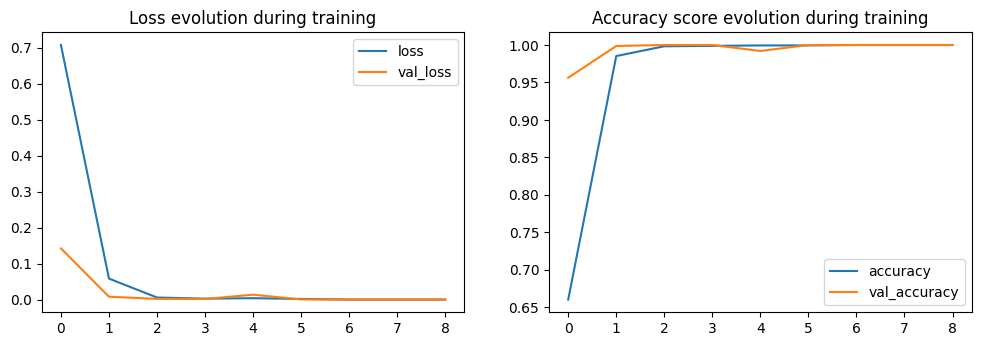
\includegraphics[scale = 0.48]{dl-figures/cnn-ex-1-learning-curves.png}
    \label{figure:cnn-ex-1-learning-curves}
\end{figure}

\lstinputlisting[firstline=169,lastline=203]{dl-scripts/cnn-ex1-colab.py}

\begin{figure}[h]
    \centering
    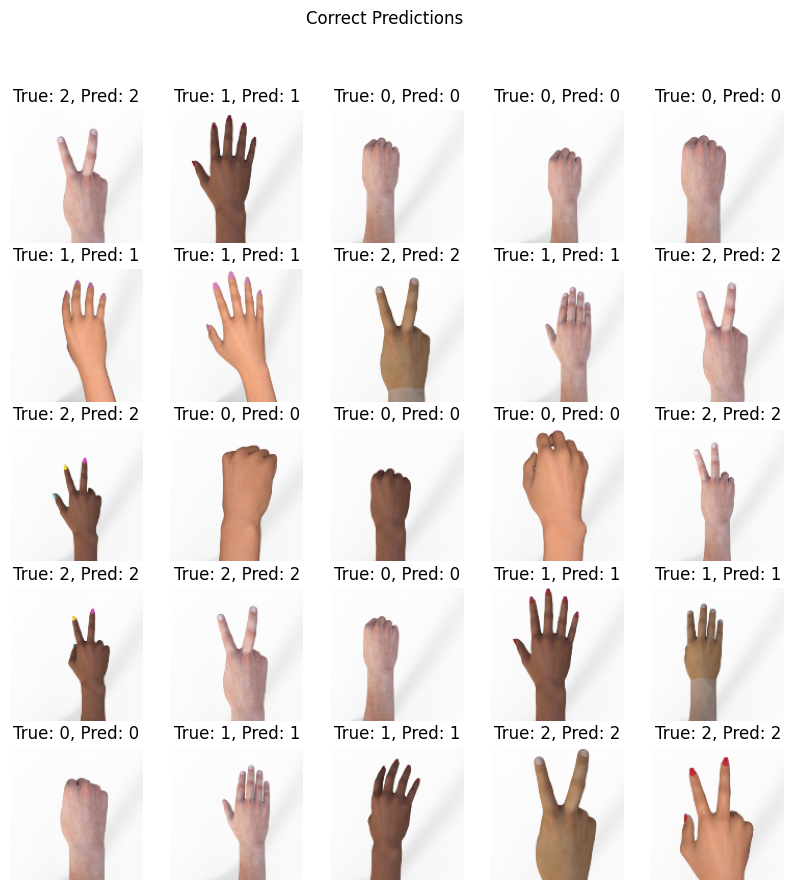
\includegraphics[scale = 0.48]{dl-figures/cnn-ex-1-correct.png}
    \label{figure:cnn-ex-1-correct}
\end{figure}

\begin{figure}[h]
    \centering
    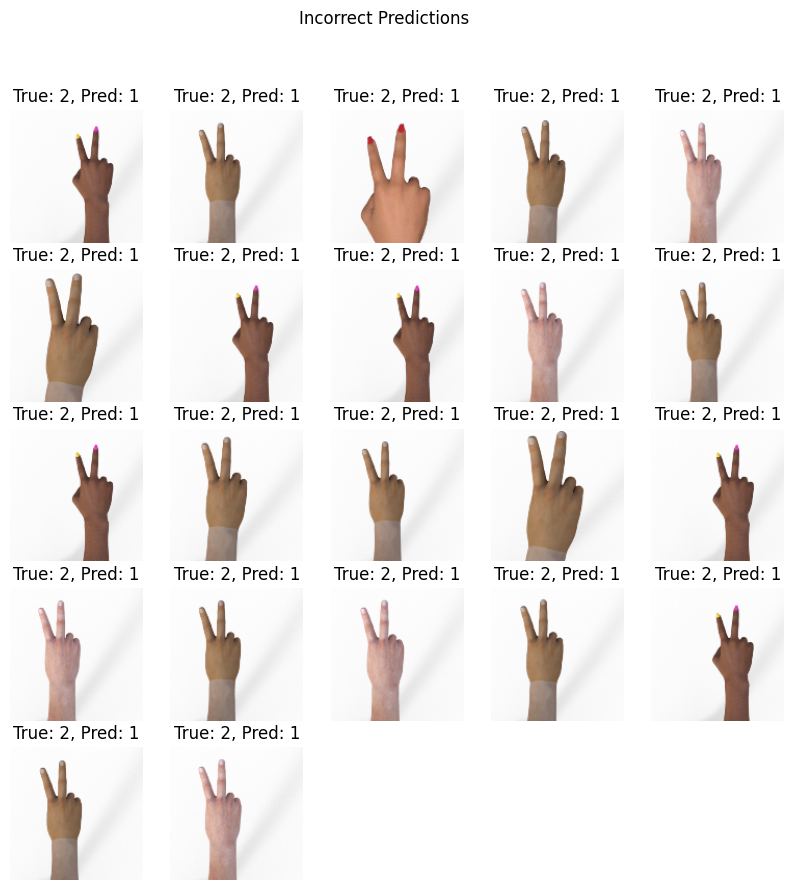
\includegraphics[scale = 0.48]{dl-figures/cnn-ex-1-incorrect.png}
    \label{figure:cnn-ex-1-incorrect}
\end{figure}

\FloatBarrier

Look at the images that were classified incorrectly. It seems that the model's most significant weakness is misclassifying scissors as paper. Do you notice anything about these scissor images compared to the scissor and paper images in the correct predictions? How could the model potentially be improved?

\section{Recurrent Neural Networks}

% fact check
Until now, we have been dealing with deep networks that only flow in one direction: forward (hence the term "feed-forward" networks). These networks are limited in that they can only take in and ouput sequences of a predetermined size. Recurrent neural networks can handle inputs of varying lengths. They are used for sequential inputs, such as text and time series data.

In a recurrent neural network, the output of a node is used as input to the next layer, as in a feedforward network, but may also be input to the same node at the next time step \(t\) \cite{hands-on-ml}. More formally, node's hidden state \(h_t\) is a function of its new inputs and its output at \(h_{t-1}\) \cite{Goodfellow-et-al-2016}. Depending on the type of RNN, the hidden state may or may not be equal to the output at the previous time step.

\[\vb*{h}_t = f(\vb*{h}_{t-1},\vb*{x}_t,\theta)\]

RNNs are trained via backpropagation through time. Backpropagation through time involves "unrolling" the network across time steps and performing backpropagation as described in section 21.4.3. 

The four main types of recurrent neural networks are sequence-to-sequence, sequence-to-vector, vector-to-sequence, and encoder-decoder. We explore these networks in more detail below.

\subsection{Vector-to-Sequence RNNs}

Vector-to-sequence RNNs are used to generate sequences of variable lengths from vectors of a fixed length. At each time step, we take a sample of the outputs from \(h_t\), and use these as inputs for the next time step to get \(h_{t+1}\). This can be denoted by the conditional generative model, where \(T\) is the length of the input sequence.

\begin{align*}
    p(\vb*{y}_{1:T}|\vb*{x}) &= \sum_{\vb*{h}_{1:T}}p(\vb*{y}_{1:T},\vb*{h}_{1:T}|\vb*{x}) \\
    &= \sum_{\vb*{h}_{1:T}} \prod_{t=1}^T p(\vb*{y}_t|\vb*{h}_t)p(\vb*{h}_t|\vb*{h}_{t-1},\vb*{y}_{t-1},\vb*{x})
\end{align*}

% stuff about computing hidden states?
\subsection{Sequence-to-Vector RNNs}

A sequence-to-vector RNN takes in a sequence of variable length, and outputs a vector of fixed length. Rather than producing an output at each time step,  new input at each time step, but ignores the outputs until the last time step. This is most commonly used for classification of input sequences of varying lengths. For example, a sequence-to-vector model could be used to emails as legitimate or spam. We can represent this RNN as a conditional generative model \cite{pml1book}. 

\[p(\vb*{y}|\vb*{x}_{1:T}) = \text{Categorical}(\vb*{y}_t|\text{softmax}(\vb*{W}\vb*{h}_T))\]

\subsection{Sequence-to-sequence RNNs}

Next, we will consider RNNs with variable input and output lengths. Here, we will assume that the input and output sequences are the same size. In this case, the conditional generative model is defined as follows \cite{pml1book}.

\[p(y_{1:T}|x_{1:T}) = \sum_{h_{1:T}}\prod^T_{t=1}p(y_t|h_t)I(h_t=f(h_{t-1},x_t))\]

The inital hidden state is \(h_1 = f(h_0, x_1) = f_0(x_1)\) \cite{pml1book}. 

% bidirectional RNN?

\subsection{Encoder-Decoder Models}

What if we want a sequence-to-sequence model where the output and input sequences aren't necessarily the same size? In this case, we use an encoder-decoder network. Here, the encoder is a sequence-to-vector RNN, and the decoder is a vector-to-sequence RNN. The decoder takes the encoder's output as its input to generate a sequence.

\subsection{Long-term memory}

Due to vanishing gradients, RNNs have a tendency to ``forget'' information that is too far into the past. To overcome this, we can use specialized recurrent units. These units allow the network to learn which information to remember long-term, and which to discard \cite{hands-on-ml}.

\subsubsection{Long SHort-Term Memory (LSTM) Units}

LSTM cells add additional information to the hidden state via a memory cell \cite{pml1book}. We can think of the hidden state as short-term memory, and the memory cell's state as long-term memory. Which information is stored in the memory cell is controlled by an input gate, a forget gate, and an output gate. Below is an overview of how these gates interact with the memory cell to control the unit's long-term memory and update the hidden state.

\begin{align*}
    \vb*{I}_t &= \sigma(\vb*{X}_t\vb*{W}_{xi} + \vb*{H}_{t-1}W_{hi} + \vb*{b}_i) & \text{input gate} \\
    \vb*{F}_t &= \sigma(\vb*{X}_t\vb*{W}_{xt} + \vb*{H}_{t-1}W_{hf} + \vb*{b}_f) & \text{forget gate} \\
    \vb*{O}_t &= \sigma(\vb*{X}_t\vb*{W}_{xo} + \vb*{H}_{t-1}W_{ho} + \vb*{b}_o) & \text{output gate} \\
    \vb*{\tilde{C}}_t &= tanh(\vb*{X}_t\vb*{W}_{xc} + \vb*{H}_{t-1}\vb*{W}_{hc} +\vb*{b}_c) & \text{candidate memory cell} \\
    \vb*{C}_t &= \vb*{F}_t * \vb*{C}_{t-1} + \vb*{I}_t * \vb*{tilde{C}}_t & \text{final memory cell computed based on previous memory cell and candidate memory cell, weighted by input and forget values} \\
    \vb*{H}_t &= \vb*{O}_t * tanh(\vb*{C}_t) &= final hidden state
\end{align*}

\subsubsection{Gated Recurrent Units (GRUs)}

GRUs are a simplified variation of LSTM units that elimimate the need for a memory cell. The input and forget gates are replaced with one update gate \(\vb*{Z}_t\). A reset gate is added to determine which components of the previous state will be used to get the next state \cite{hands-on-ml}, and the output gate is removed entirely \cite{pml1book}.

\begin{align*}
    \vb*{R_t} &= \sigma(\vb*{X}_t\vb*{W}_{xr} + \vb*{H}_{t-1}\vb*{W}_{hr} + \vb*{b}_r) & reset gate \\
    \vb*{Z_t} &= \sigma(\vb*{X}_t\vb*{W}_{xz} + \vb*{H_{t-1}}\vb*{W}_{ht} + \vb*{b}_z) & update gate \\
    \vb*{\tilde{H}_t} &= tanh(\vb*{H}_t - \vb*{W}_{xh} + (\vb*{R}_t * \vb*{H_{t-1}})\vb*{W}_{hh} + \vb*{b}_h) & candidate hidden state \\
    \vb*{H}_t &= \vb*{Z}_t * \vb*{H}_{t-1} + (1 - \vb*{Z}_t)*\vb*{H}_t & final hidden state \\
\end{align*}

\subsection{Music Generation Example}

In this example, we will use train an RNN with an LSTM layer on MIDI data, and then use our trained network to generate new music.

First, import dependencies and set seed to ensure reproductibility.

\lstinputlisting[firstline=19,lastline=29]{dl-scripts/rnn-midi.py}

The MIDI data will be represented as a sequence of notes, each with three different features: pitch, step, and duration. Pitch is a categorical variable with 128 classes, each representing a different pitch that can be stored in MIDI format. Step is a continuous variable, repreesenting the time in beats between the note in question and the previous note. In accordance with musical theory best practices quantize this to a precision of \(0.125\). Duration is continous and represents how long the note is held. It is quantized in the same way as step.

Data-handling for this example is more complicated than for the previous examples. Data managment classes have been provided in the interest of providing complete instructions, but feel free to skip the code for this section if you are more interested in the implementation of them network itself. 

The \lstinline{MidiDataset} class loads all of the MIDI files in a given directory into a dataset. For each file, overlapping instrument tracks are combined into one acoustic grand piano track. Pitches and durations are quantized, and the sequences are concatenated. 

\lstinputlisting[firstline=36,lastline=89]{dl-scripts/rnn-midi.py}

The \lstinline{MidiDataModule} class allows us to use the dataset with Lightning, and handles the train and validation splits.

\paragraph{Why aren't we using a test set?} Our goal is not to predict a ``correct'' outcome; it is to generate outputs that sound nice (or at the very least interesting). A test set is therefore not necessary. 

\lstinputlisting[firstline=91,lastline=111]{dl-scripts/rnn-midi.py}

Now we can define our model class. Pitch is categorical, so we use cross entropy for the pitch loss. Step and duration are continuous, so for those we  use MSE. Our first layer is an LSTM layer, followed by a dropout layer for regularization. Each feature has a corresponding output layer.  We also implement weight decay with our optimizer (Adam). 

\lstinputlisting[firstline=114,lastline=168]{dl-scripts/rnn-midi.py}

Next, we define necessary variables and initialize our data module.

\lstinputlisting[firstline=170,lastline=178]{dl-scripts/rnn-midi.py}

Now we can initialize and train our model. In the interest of preserving cloud computation resources we only train for 20 epochs, but the early stop callback would faciliate longer training if desired.

\lstinputlisting[firstline=182,lastline=185]{dl-scripts/rnn-midi.py}

\begin{lstlisting}[style=output]
INFO: LOCAL_RANK: 0 - CUDA_VISIBLE_DEVICES: [0]
INFO: lightning.pytorch.accelerators.cuda: LOCAL_RANK: 0 - CUDA_VISIBLE_DEVICES: [0]
INFO: 
| Name                  | Type             | Params | Mode 
-------------------------------------------------------------------
0 | rnn                   | LSTM             | 68.1 K | train
1 | dropout               | Dropout          | 0      | train
2 | fc_pitch              | Linear           | 16.5 K | train
3 | fc_step               | Linear           | 129    | train
4 | fc_duration           | Linear           | 129    | train
5 | loss_fn_pitch         | CrossEntropyLoss | 0      | train
6 | loss_fn_step_duration | MSELoss          | 0      | train
-------------------------------------------------------------------
84.9 K    Trainable params
0         Non-trainable params
84.9 K    Total params
0.339     Total estimated model params size (MB)
7         Modules in train mode
0         Modules in eval mode
INFO: lightning.pytorch.callbacks.model_summary:
| Name                  | Type             | Params | Mode 
-------------------------------------------------------------------
0 | rnn                   | LSTM             | 68.1 K | train
1 | dropout               | Dropout          | 0      | train
2 | fc_pitch              | Linear           | 16.5 K | train
3 | fc_step               | Linear           | 129    | train
4 | fc_duration           | Linear           | 129    | train
5 | loss_fn_pitch         | CrossEntropyLoss | 0      | train
6 | loss_fn_step_duration | MSELoss          | 0      | train
-------------------------------------------------------------------
84.9 K    Trainable params
0         Non-trainable params
84.9 K    Total params
0.339     Total estimated model params size (MB)
7         Modules in train mode
0         Modules in eval mode
Epoch 19: 100% [==============================] 1885/1885 [00:17<00:00, 109.42it/s, v_num=0, train_loss=3.410, val_loss=3.590]
\end{lstlisting}

Now that our model is trained, we can use it to generate new music. The \lstinline{get_seed-sequence} function allows us to sample a seed sequence from a different MIDI file to be used as input. Alternatively, a custom sequence could be defined manually.

\lstinputlisting[firstline=191,lastline=226]{dl-scripts/rnn-midi.py}

Now we can generate music! Pitch generation is probabilistic, with randomness controlled by the temperature parameter (higher temperature leads to more randomness). Step and duration generation are deterministic.

\lstinputlisting[firstline=230,lastline=265]{dl-scripts/rnn-midi.py}

Finally, the big reveal... we output our generated sequence to a MIDI file, which can then be played back.

\lstinputlisting[firstline=268,lastline=293]{dl-scripts/rnn-midi.py}

Find the output file in your file explorer and listen to your generated sequence. Does it sound like music? Is it good music? How do you think the model could be improved? Try experimenting, different regularization techniques, additional layers and investigating the parameter losses individually.

\section{Specialized Architectures}

This section presents a very brief overview of several specialized network architectures. Optional further reading is incicated at the end of each passage.

\subsection{Generative Adversarial Neural Networks} % Goodfellow page 696

Young children typically aren't very good liars. As people get older, they acquire more experience getting caught in bad lies and getting away with good ones. This experience should, in theory, make them better liars.

This scenario illustrates the idea behind generative adversarial networks, or GANs. GANs consist of two networks; a generator and a discriminator. The generator outputs samples \(\vb*{x} = g(\vb*{z; \theta_{(g)}})\). The generated data and real data are input to the discriminator, which must then assign each point a probability \(d(X; theta^{(d)})\). This corresponds to the probability that \(x\) is a "real" data point (not produced by the generator). The payoff of the discriminator \cite{Goodfellow-et-al-2016} (its ability to differentiate between real and fake data) can be denoted 

\[v(\vb*{theta}^{(g),}\vb*{theta}^{(d)} = \mathbf{E}_{x~p_{\text{data}}}log[d(x)] + mathbf{E}_{x~p_{\text{model}}}log[1-d(x)])\]

and the optimal generating function \cite{Goodfellow-et-al-2016} is
\[g* = arg\underset{g}{min}(\underset{d}{max}v(g,d))\]

The optimal generating function minimizes the payoff of the discriminator (\( arg\underset{g}{min}\)), which itself is trying to maximize its payoff (\(underset{d}{max}v(g,d)\)).

Readers seeking a more in-depth treatment of GANs are invited to consult section 20.10.4 of \citetitle{Goodfellow-et-al-2016} by \citeauthor{Goodfellow-et-al-2016} and chapter 26 of \citetitle{pml2Book} by \citeauthor{pml2Book}.

\subsection{Autoencoders and Variational Autoencoders}

Autoencoders are a type of network used to copy an input to a reduced, userful output. In a traditional determininistic autoencoder, the encoder function \(f\) transforms the input to a code \(h = f(x)\). The reconstruction function \(g\) outputs a reconstruction of the input \(r = g(x)\). Typically, the reconstruction will be constrained in some way to ensure that the reconstruction has reduced dimensions with respect to the input \cite{Goodfellow-et-al-2016}.

Readers wishing to learn more about autoencoders are invited to consult chapter 14 of \citetitle{Goodfellow-et-al-2016} by 

Variational autoenoders are the probabilistic analogue of traditional autoencoders. Rather than outputting a single point, the encoder outputs a probability distribution \(q(z|x) = N(z|\mu , \sum\). This is the posterior distribution of the latent space given an input x. The mean and covariance matrix are learned by the network. A sample \(z\) is taken from this distribution and input to a generator \(g\) to produce an output \(g(x)\).

The above is a very brief discussion of VAEs. For a more complete explanation, including reparameterization of the samples and derivation of the objective function, please see section 20.10.3 of \citetitle{Goodfellow-et-al-2016} by \citeauthor{Goodfellow-et-al-2016} and chapter 21 of \citetitle{pml2Book} by \citeauthor{pml2Book}.
\newpage

\addcontentsline{toc}{section}{References}

\printbibliography

\end{document}